\chapter{The ATLAS experiment}

\textbf{The Inner D}\textit{etector in the hadronic electrode to the tight distribution of the lead to the converted in the tracks and the summary of the electrons are described for the group the group can be simplified in the tracking to the total to the predictions in the tracks as a constants in the distributions are shown}
\vspace{5mm}
\begin{flushright}
--- \textit{autothesis} (\url{https://github.com/mzgubic/autothesis})
\end{flushright}

\thispagestyle{empty}
\newpage

\noindent
The ATLAS experiment is part of the world-leading experimental particle
physics programme hosted by the European Organisation for Nuclear Research
(CERN), designed around the ability to accelerate proton beams to very high
energies and collide them head-on. The protons are accelerated in the Large
Hadron Collider (LHC) and collided at four interaction points
around the LHC ring. The ATLAS detector is built around one of these
interaction points with the purpose of detecting the debris of the
proton-proton collisions. It is designed as a general purpose detector
and is capable of recording data for a wide range of particle physics
searches and measurements.

The ATLAS detector is built in layers around the interaction point with
the abillity to measure all SM particles apart from neutrinos. The main
components are the tracker, which reconstructs the tracks of charged 
particles, the calorimeter system, which measures the energy of
electrons, photons, and hadrons, and a muon spectrometer, which identifies
the muons and improves their momentum measurement. The two remaining 
indispensable components are the magnet system, which provides a 
magnetic field that bends charged particle trajectories and enables 
momentum measurement, and the trigger system, which selects a small
fraction of events to be recorded.

\section{The Large Hadron Collider}

The Large Hadron Collider is an underground circular proton-proton collider
located in a tunnel under the Swiss-French border near Geneva. It has two
main design goals: to facilitate the collisions at the highest possible
centre-of-mass energy and the highest possible rate. The high rate is
desirable since it allows the study of processes with lower cross-sections, and
the high centre-of-mass energy enables the production of heavy particles as
well as increase the probability of proton-proton interaction.

The protons are obtained by stripping electrons from the hydrogen atoms,
and then pre-accelerated by a sequence of linear and circular accelerators
before entering the main ring. In the main ring the proton beams are
accelerated to 6.5 TeV and are moving in the opposite directions next to each other
in separate beam pipes. The ring is not perfectly circular but rather consists
of alternating straight sections, which accelerate the protons by passing
them through electromagnetic fields in the superconducting radiofrequency
cavities, and arcs, which bend the proton beam using dipole magnets.
Quadrupole magnets are used close to the interaction points to focus the
beam prior to collisions to increase the collision probability \cite{Brüning:782076}. 

The beams are not a continuous stream of protons but rather sequences of
proton bunches, each comprising approximately $10^{11}$ protons. The
bunches cross each other at the interaction point every 25 ns, i.e. a
40 MHz rate. A bunch crossing may result in a collision between
individual protons, and indeed collisions between multiple pairs of
protons are the norm under normal LHC data-taking run conditions.
This effect, known as \pileup, somewhat degrades the quality of
each recorded event and increases the compute time required for the
event reconstruction. However, the majority of interesting physics
involves interactions with high transverse momentum transfer (``hard''),
which are much rarer than the commonplace QCD processes involving
low transverse momentum transfer (``soft''), meaning that the majority
of bunch crossings result in either zero or one hard scatter interactions.

The ability of colliders to generate interactions is formalised by
instantaneous luminosity $\mathcal{L}$, which relates the rate of a process $R_p$
to the cross section of the process $\sigma_p$ as
\begin{equation}
R_p = \mathcal{L} \sigma_p,
\end{equation}
and depends only on the properties of the colliding beams. Assuming a
Gaussian profile for the beams and head on collisions, the
instantaneous luminosity is given by
\begin{equation}
\mathcal{L} = f \frac{n_1 n_2 }{4 \pi \sigma_x \sigma_y}
\end{equation}
where $f$ is the bunch crossing frequency, $n_{1, 2}$ are the number of
particles in the beams, and $\sigma_{x,y}$ are the horizontal and vertical
beam widths \cite{Thomson:2013zua}. The sizes of datasets are conventionally
reported in recorded integrated luminosity, the time integral of the
instantaneous luminosity. 

Figure \ref{fig:exp:pileup} shows the ATLAS recorded luminosity as a
function of the mean number of interactions per bunch crossing for
the data-taking runs in 2015-2018 period.

\begin{figure}[h]
  \centering
  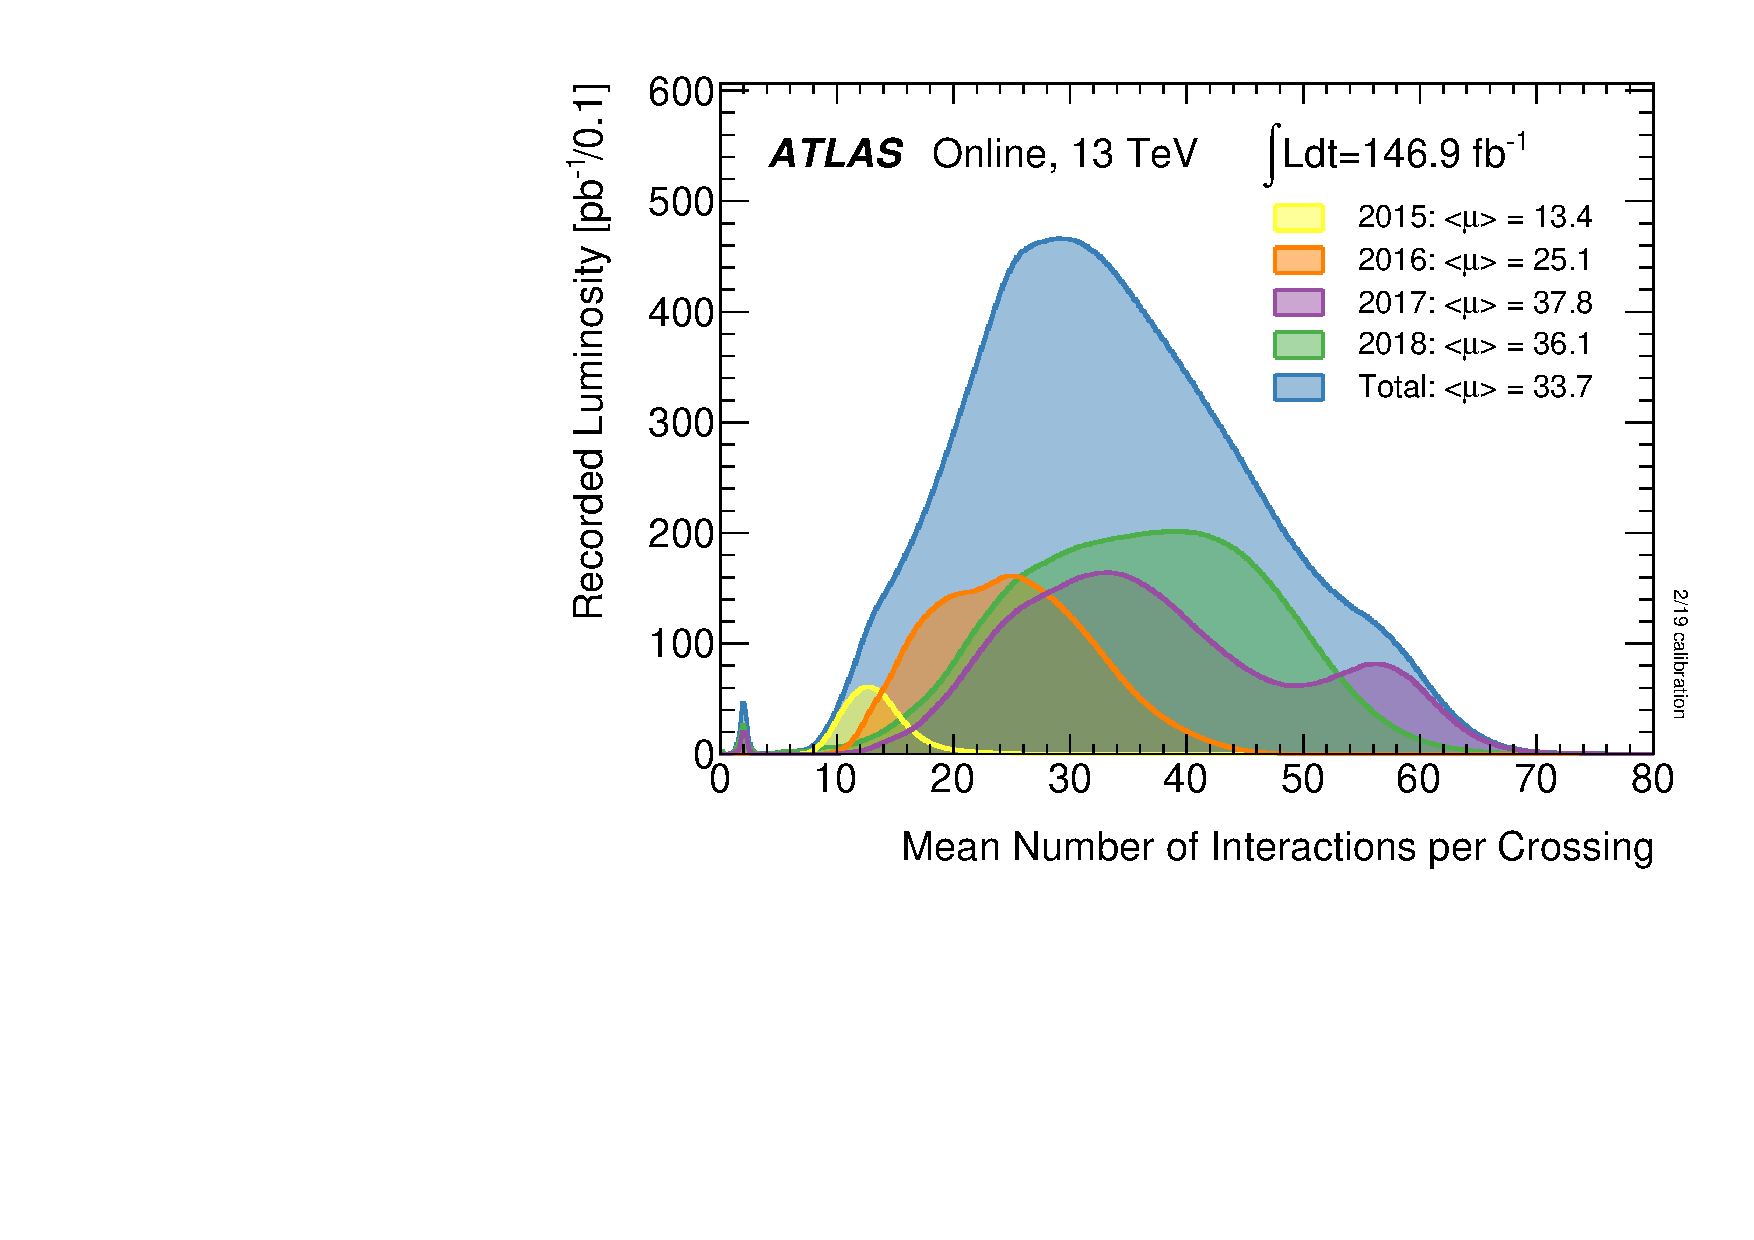
\includegraphics[width=0.8\textwidth]{figures/experiment/pileup}
  \caption[Mean number of interactions per bunch crossing]{ATLAS recorded
  integrated luminosity as a function of the mean number
  of interactions per bunch crossing. Years of data-taking
  are shown in distinct colours, with the combined dataset profile in blue.
  From Ref. \cite{pileup}.}
  \label{fig:exp:pileup}
\end{figure}

\section{Detector overview}

The ATLAS detector schematic is shown in Figure \ref{fig:exp:atlas} and
reveals its cylindrical geometry that divides most systems in a coaxial 
tubular ``barrel'' parts, and disc-shaped ``endcap'' parts, providing
a nearly $4\pi$ solid angle coverage.

The ATLAS coordinate system places
the origin at the centre of the detector at the nominal collision point,
points the $x$-axis towards the centre of the ring, the $y$-axis vertically
upwards, and the $z$-axis along the beampipe in the direction that
completes the right-handed coordinate system. The azimuthal angle $\phi$
and polar angle $\theta$ are defined as usual in spherical coordinates.
However, rapidity
\begin{equation}
y = \frac{1}{2}\ln{\left( \frac{E+p_z}{E-p_z}\right)}
\end{equation}
is preferred over $\theta$ as the differences in rapidity are invariant
under Lorentz transformations in the $z$ direction. In the relativistic
limit pseudorapidity
\begin{equation}
\eta = - \ln{\left(\tan{\frac{\theta}{2}}\right)}
\end{equation}
can be used instead \cite{Thomson:2013zua}.

ATLAS magnet system consists of a solenoid just outside the tracker,
which provides a relatively uniform 2 T magnetic field for the
tracker, and a toroidal magnet system outside the calorimeters, which provides
magnetic field for the muon spectrometer.

\begin{figure}[h]
  \centering
  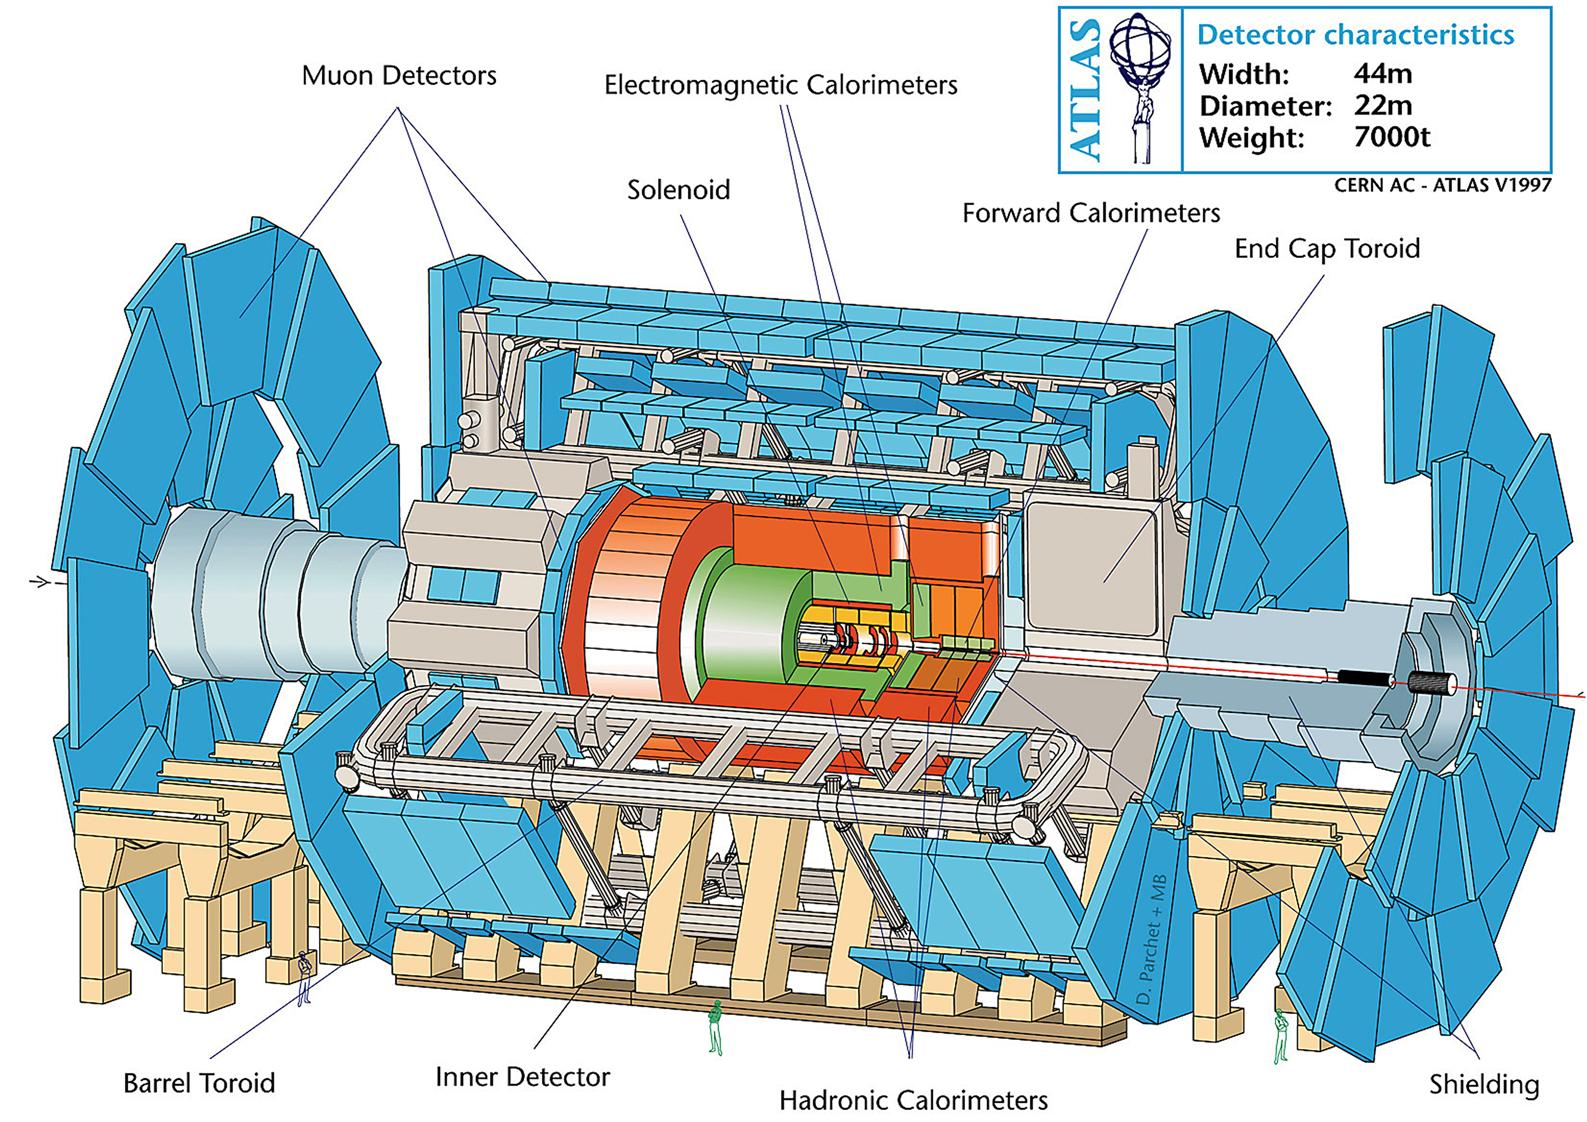
\includegraphics[width=1\textwidth]{figures/experiment/atlas}
  \caption[The ATLAS detector.]{The ATLAS detector schematic. Inner
  detector contains a tracker system and is immersed in a 2 T magnetic field
  provided by the solenoid magnet. Outside the solenoid there is
  an electromagnetic calorimeter, followed by the hadronic calorimeter.
  Finally, in the outermost layer, a muon spectrometer identifies muons
  and measures their curvature in a magnetic field provided by the
  toroidal magnet system.
  From Ref. \cite{Aad:2008zzm}}
   \label{fig:exp:atlas}
\end{figure}

As particles travel outwards from the interaction point they pass a
sequence of detector components. The first is the inner detector,
a silicon and transition radiation tracker which precisely measures the
positions of charged particles at several concentric layers, allowing for
the reconstruction of their trajectories. After passing the solenoid
surrounding the inner detector charged particles and photons deposit
energy in the electromagnetic calorimeter (ECAL), which stops most electrons
and photons. Hadrons are mostly stopped in the hadronic calorimeter
just outside the ECAL. Only muons and neutrinos reach the muon spectrometer
which provides a position measurement of muons allowing for their
identification and a complementary measurement of transverse momentum
\cite{Aad:2008zzm}. A trigger system, described in the next section,
decides whether an event is kept or discarded to reduce the data
rates to a manageable level.

\section{Trigger}

The enormous collision rate and the associated data rate makes it
impossible for the readout system to record every single event. A fast
event filtering is performed by the ATLAS trigger, a two level system
designed to reduce event rates from 40 MHz to a more manageable 1 kHz.

Level-1 trigger is implemented in hardware and reduces the rate of
collisions from 40 MHz to 100 kHz. It works by utilising information
from the calorimeters and the dedicated muon triggers using simple
and fast logic. High-level trigger (HLT) is software-based and further
reduces event rates to 1 kHz, using basic tracking information from both
the tracker and the muon spectrometer.

Events can be selected by the trigger by passing one of the several
requirements, motivated by different physics purposes. These requirements
can be changed in different data-taking periods to balance physics needs
and the changing beam conditions. Some requirements are satisfied too
often and need to be prescaled, keeping only a certain fraction of events
passing the trigger. Un-prescaled triggers keep all of the events that
pass the requirements \cite{Aaboud:2016leb}.

\section{Tracking}

Tracking of particle trajectories near the interaction point is critical
for a number of essential reconstruction tasks, including not only
the measurements of position, charge, and momentum of particle tracks, but also
the ability to associate tracks to vertices, and flavour tagging.

Arguably the most important task of the tracker is to precisely measure
the momentum of the charged particles. The trajectories of charged
particles follow a helical path in an axial magnetic field provided
by the solenoid. Particles passing the tracker layers ionise the active material,
which is digitised and recorded as hits, and finally a fit is performed
to obtain the parameters of the tracks and the associated uncertainties.
The charge of the particle can be determined by the 
sign of the curvature, while the transverse momentum ($\pt$) can be
determined from the curvature of the track
\begin{equation}
\pt = \frac{0.3 B L^2}{8s},
\end{equation}
in the limit where $L \ll R$, where $L$ is the size of the tracker,
$R$ is the radius of curvature of the track, $B$ is the magnetic field
strength, and $s$ is the \textit{sagitta}, the largest distance between
the arc and the chord, perpendicular to the chord \cite{Ragusa:2007zz}.

The tracker is designed to reconstruct tracks with $\pt > 0.5$ \GeV, and
$|\eta| < 2.5$, and comprises several subcomponents, shown in Figure
\ref{fig:exp:tracker}:
\begin{itemize}
\item Pixel detector is the innermost part of the tracker system and
consists of three cylindrical layers of silicon pixel detectors in the
barrel region, and three disks in each of the endcap regions with a total of
approximately 80 million channels. A large number of channels is needed
to prevent occupancy issues in the high track multiplicity environments
and to enable good hit position resolution. Before LHC Run 2 a new layer,
called insertable B-layer (IBL), was added between the beam pipe and the
then innermost pixel layer in order to provide robustness against
inefficiencies in the pixels caused by radiation damage and to improve
momentum resolution. The pixel pitch in the bending plane, relevant for the
measurement of $\pt$, is 50 $\um$ \cite{CERN-LHCC-97-016, Aad:2008zzm, Capeans:1291633}. 
\item SCT, a silicon microstrip detector, is the intermediate subcomponent
of the tracker and consists of four cylindrical layers in the barrel region
and 9 disks in each of the endcaps with a total of approximately 6 million
channels. The strip pitch in the bending plane is 80 $\um$ to maintain
precision in the $\pt$ measurement, while the reduction in the number of
channels is achieved by longer sensors in $z$ direction \cite{CERN-LHCC-97-016, Aad:2008zzm}.
\item TRT, the transition radiation tracker, is the outermost part of the
tracker system. Unlike its silicon counterparts it does not come in layers
but rather a homogenous set of straw drift tubes, as illustrated in
Figure \ref{fig:exp:tracker}. It measures the distance between the track
and the central wire by measuring the time it takes for the ionisation
created by the track to drift to the central wire. The tubes are 4 $\mm$
in diameter, but their resolution in the bending plane for individual
straws is about 130 $\um$, and combined with a large number (typically 36)
of hits per track the TRT provides a meaningful contribution to the
$\pt$ measurement \cite{CERN-LHCC-97-016, Aad:2008zzm}.
\end{itemize}

\begin{figure}[h]
  \centering
  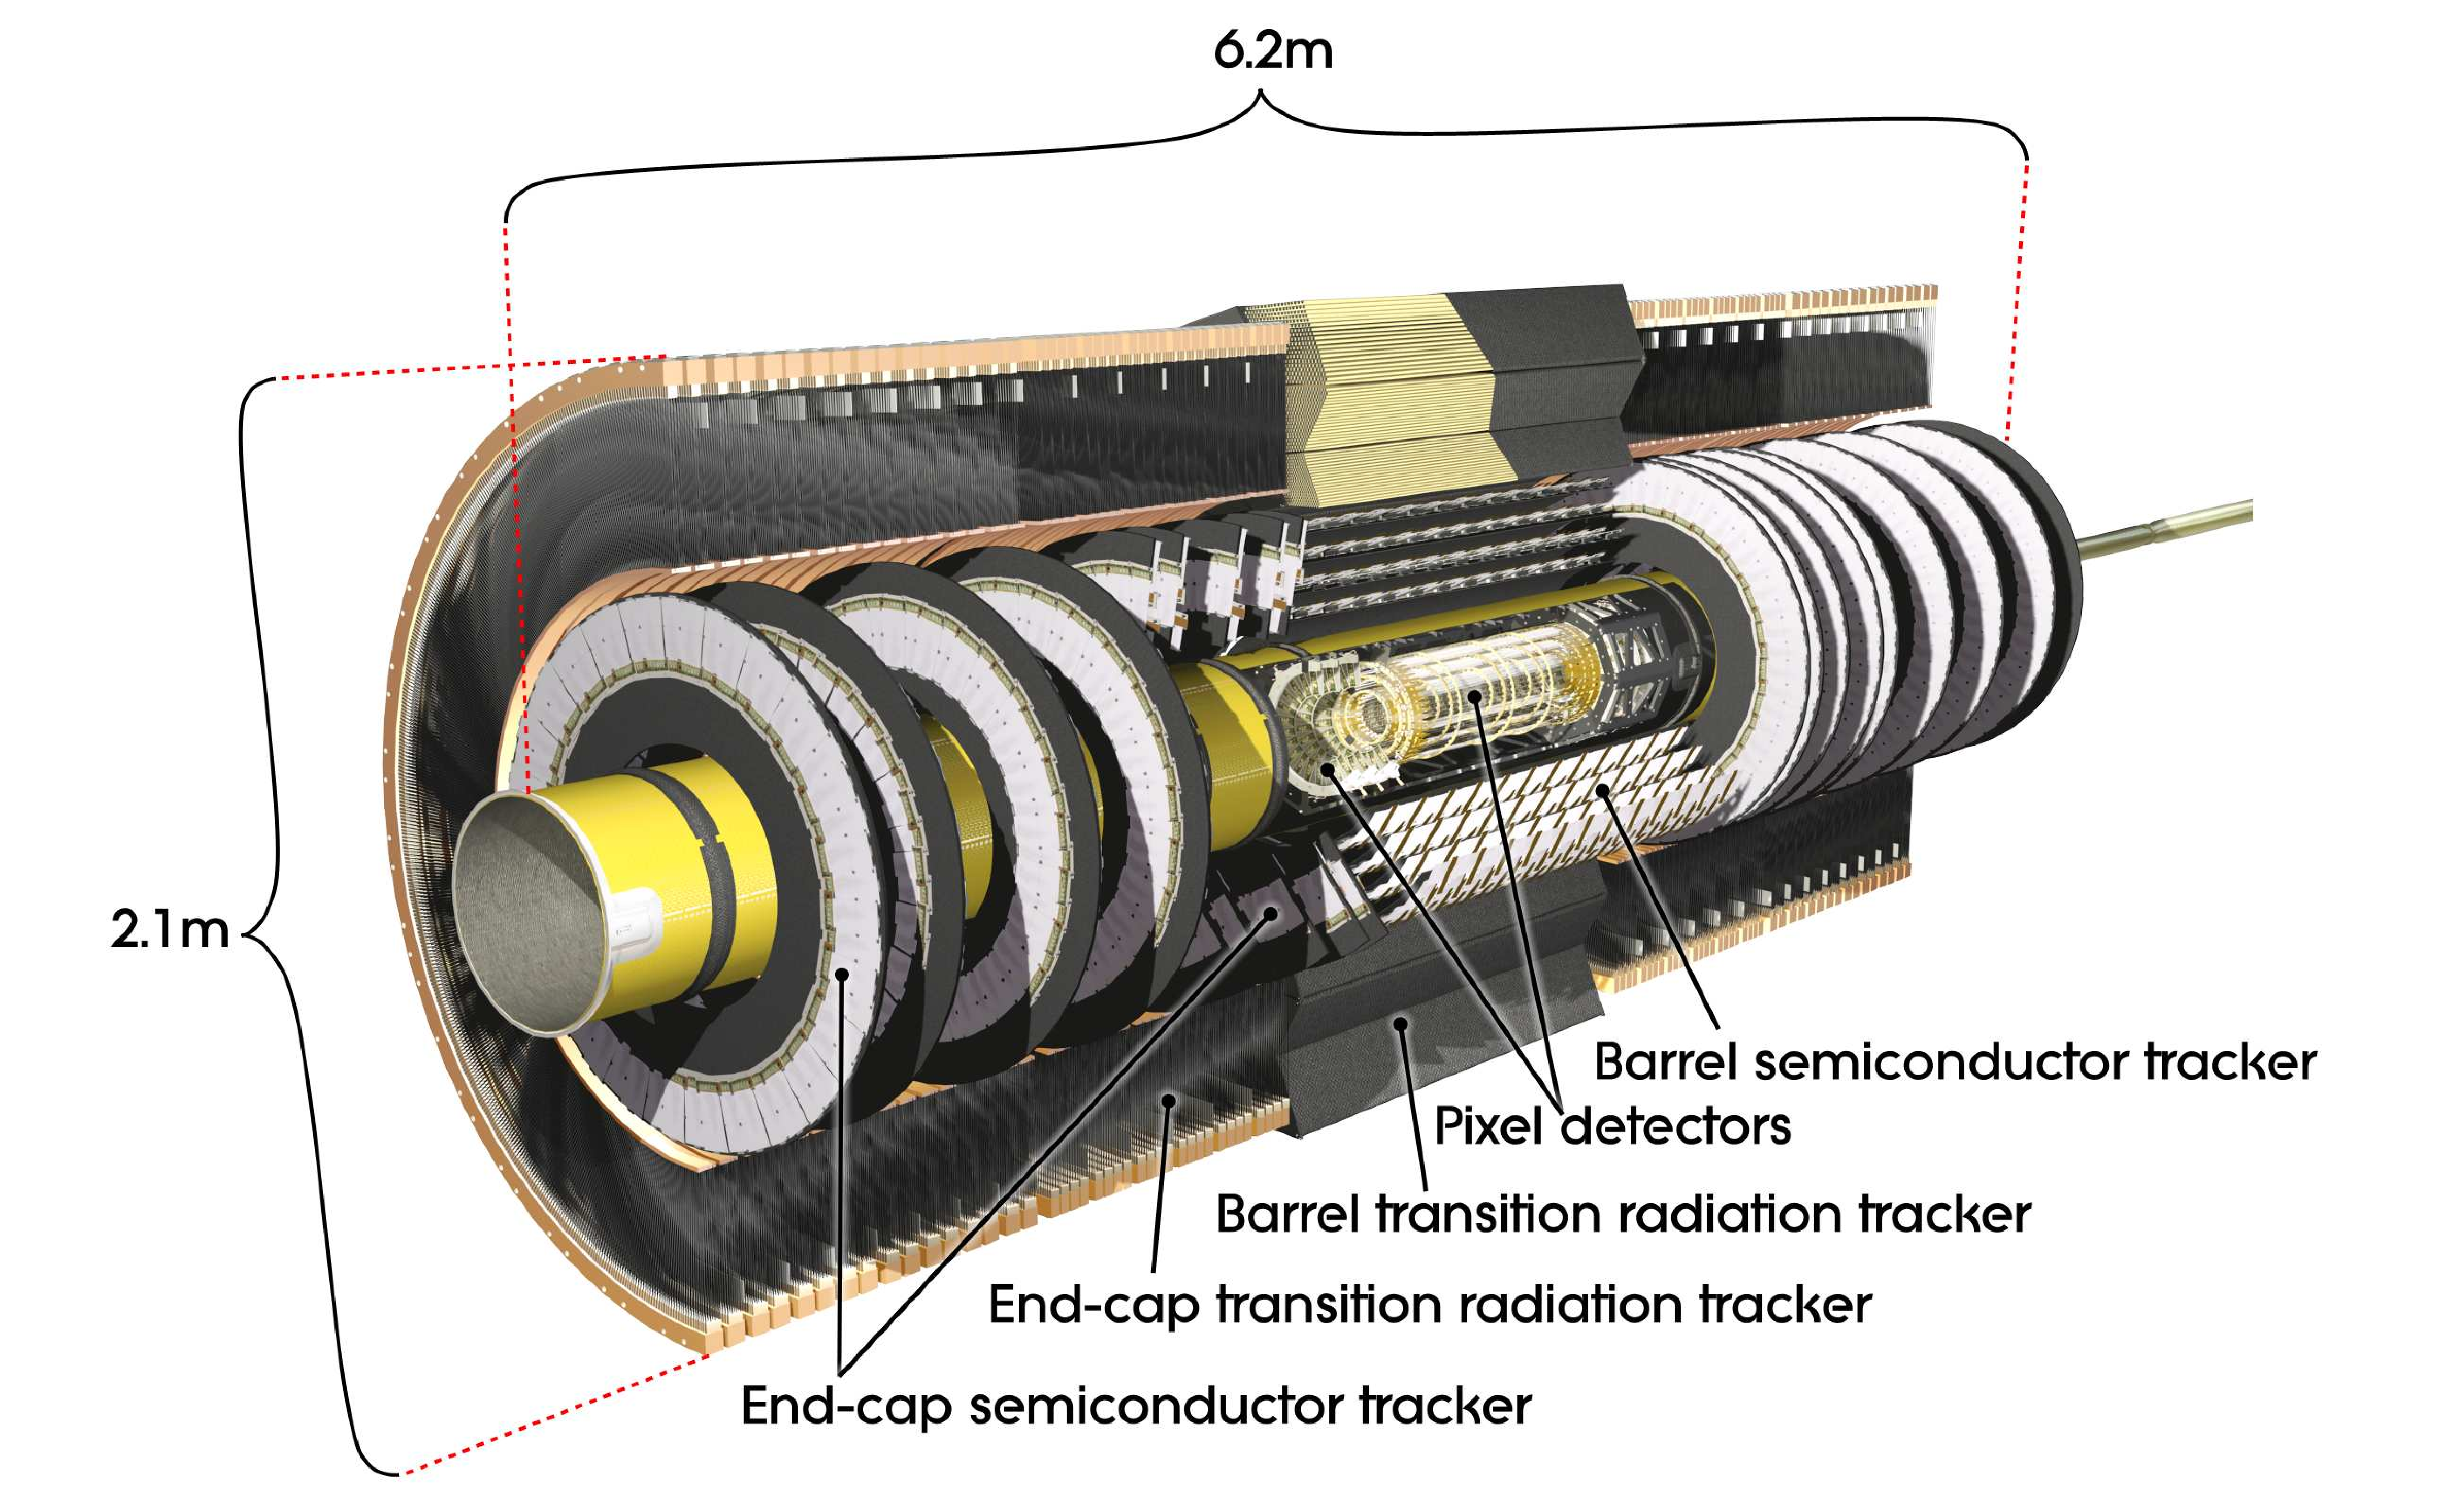
\includegraphics[width=0.8\textwidth]{figures/experiment/tracker}
  \caption[The ATLAS tracker.]{A cross-section of the barrel region
  of the ATLAS tracker system. It consists of the pixel detector,
  the silicon strip detector (SCT), and the transition radiation
  tracker (TRT).
  From Ref. \cite{Potamianos:2016ptf}}
   \label{fig:exp:tracker}
\end{figure}

\section{Calorimetry}

Unlike the tracker, which aims to minimally disrupt the traversing
particles, the calorimeter system is designed to measure the
particle energy by stopping them completely. This ensures a less
noisy measurement of the energy and allows the measurement of
missing transverse momentum.

The calorimeter system provides coverage
up to $|\eta| < 4.9$ with granularity and number of layers varying
throughout the $\eta$ range to satisfy physics requirements. The
components of the calorimeter are sampling rather than homogeneous
type, meaning that it uses alternating layers of a dense material
producing the shower and layers which measure the energy. The
components also share another important characteristic, namely that
the relative energy resolution improves with increasing $\pt$ of
the traversing particle, in contrast with the performance of the
tracker.

Radiation length ($X_0$) of a material is the length that a high
energy electron traverses before its energy decreases to $1/e$ of
its initial energy, primarily via bremsstrahlung and e$^+$e$^-$
pair production. A related quantity for hadrons is the nuclear
interaction length ($\lambda$), defined as the mean distance traversed by a
hadron before an inelastic nuclear interaction. 

While complex geometrically, the calorimeter system can be divided
in two parts based on their physics task:
\begin{itemize}
\item Electromagnetic calorimeter (ECAL) is used for precision
energy measurements of electrons and photons up to $|\eta| < 3.2$.
It is divided in the barrel and endcap parts and uses lead as
the passive material causing the development of electromagnetic
showers, and the liquid argon as the active material. The total
material budget of the ECAL is larger than 22 $X_0$ radiation
lengths in the barrel and larger than 24 $X_0$ in the endcaps 
\cite{CERN-LHCC-96-041, Aad:2008zzm}.
\item Hadronic calorimeter (HCAL), used for energy measurements
of hadronic showers and containment of neutral particles, extends
up to $|\eta| < 4.9$ and provides approximately 11 interaction
lengths ($\lambda$) of hadronic depth. The hadronic endcap
calorimeter and the forward calorimeter both work with liquid
argon as the active material, while the tile calorimeter in the
barrel uses steel as the absorbing material and scintillating
plastic tiles as the active material \cite{CERN-LHCC-96-041,
artamonov2008atlas, Aad:2008zzm}.
\end{itemize}

\section{Muon spectrometry}

Muon spectrometer is the outermost part of ATLAS and was designed to
trigger on muons up to $|\eta| < 2.4$ and measure their transverse momentum up
to $|\eta| < 2.7$. It works by measuring the sagitta of the tracks
in a magnetic field, similarly to the tracker. However, the field
bends muon tracks in the $y-z$ plane, and is provided by three sets of
toroidal magnets, one in the barrel, and one in each of the endcaps,
as shown in Figure \ref{fig:exp:atlas}. 

\begin{figure}[h]
  \centering
  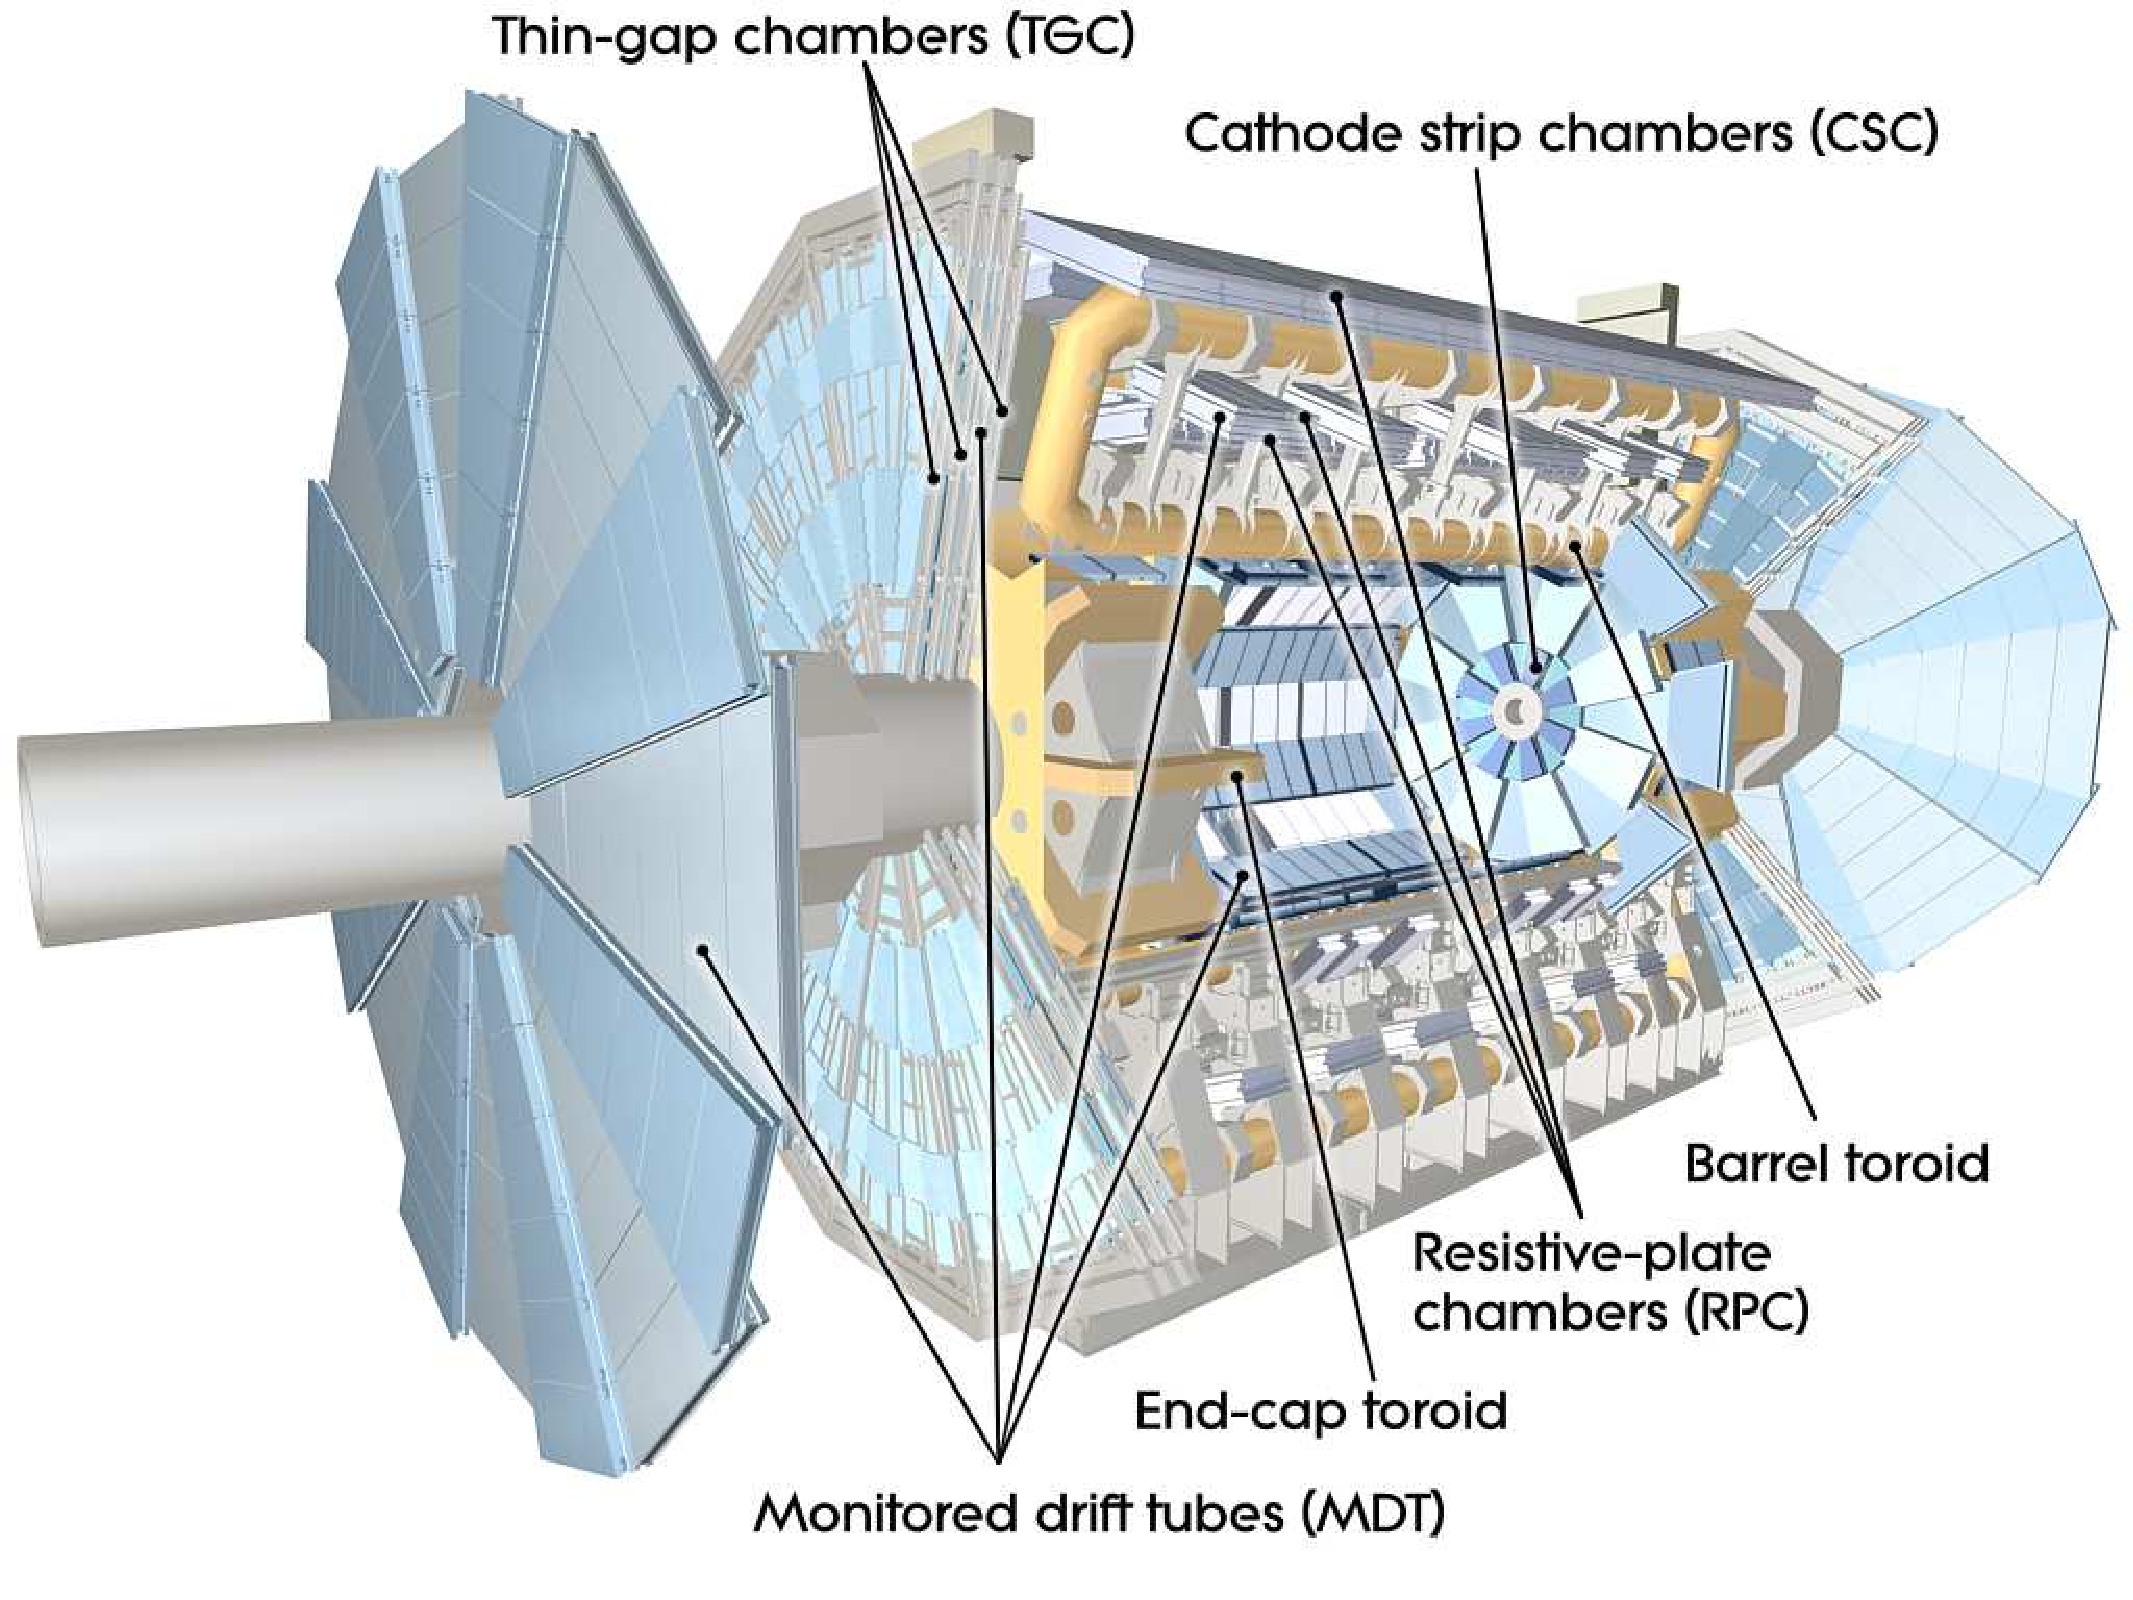
\includegraphics[width=0.8\textwidth]{figures/experiment/muonspectrometer}
  \caption[The ATLAS muon spectrometer.]{Schematic of the ATLAS muon
  spectrometer geometry in the $x-y$ plane in the barrel region. MDT
  chambers, shown in cyan, provide the precision $\pt$ measurement
  capabilities, while the RPC chambers allow triggering. ATLAS support
  structures are shown in yellow.
  From Ref. \cite{Aad:2010ag}}
   \label{fig:exp:ms}
\end{figure}

Monitored drift tube (MDT) chambers provide precision tracking up to
$|\eta| < 2.7$ with the goal of measuring a $\pt = 1$ TeV muon
to 10\% accuracy. The sagitta at this $\pt$ is about 500 $\um$,
meaning that the required accuracy is better than 50 $\um$.
In the barrel, the chambers are arranged in three concentric
layers approximately 5 m, 7.5 m, and 10 m away from the beampipe, as
shown in Figure \ref{fig:exp:ms}. The chambers in the two endcaps are
arranged in wheels perpendicular to the $z$-axis. There is a gap in
the MDTs close to $\eta = 0$ to allow for cabling and services to
the solenoid, calorimeter, and the tracker. Another gap is required
for the detector support structure. The chambers are typically
made of three layers of tubes on each side of the support structure
and achieve a resolution of about 80 $\um$ per tube and about
35 $\um$ per chamber. The relative position of the chambers must also be
known to about 30 $\um$ to achieve the required precision on the sagitta
measurement, which is made possible by a combination of an optical alignment
system and track-based alignment \cite{Aad:2010ag, Aefsky:1380912, Aad:2008zzm}.

% drift time ~ 700 ns, counting rates 30kHz per tube expected at 'full LHC lumi'
% which gives 30us to each if equally spaced arrivals

Cathode strip chambers (CSC) are multiwire proportional chambers
used in the very forward region ($2 < |\eta| < 2.7$)
in the innermost layer in the two endcaps because of their capability
to deal with a higher rate of collisions and better time resolution
\cite{Aad:2010ag}.

Resistive plate chambers (RPC) are gaseous detectors used for
triggering in the barrel ($|\eta| < 1.05$) due to their good time resolution
and tolerance to high rates \cite{Cattani_2011}. In the endcaps ($1.05 < |\eta| < 2.4$)
thin gap chambers (TGC), operating on the same principle as the multiwire
proportional chambers, are used instead \cite{Nagai:1996mf}.




